\documentclass[a4paper,11pt]{article}
\usepackage{geometry}
\geometry{margin=1in, headheight=15pt}
\usepackage{amsmath}
\usepackage{amssymb}
\usepackage{mathtools}
\usepackage{graphicx}
\usepackage{xcolor}
\definecolor{blue3}{RGB}{0,0,180}
\definecolor{green3}{RGB}{0,120,0}
\definecolor{orange3}{RGB}{200,100,0}
\usepackage{siunitx}
\sisetup{detect-all}
\usepackage[colorlinks=true,linkcolor=blue3,citecolor=blue3,urlcolor=blue3]{hyperref}
\usepackage{cleveref}
\usepackage{tcolorbox}
\tcbuselibrary{skins,breakable}
\newtcolorbox{derivationbox}[1][]{colback=blue!10,colframe=blue3,coltitle=blue3,title={Derivation:},fonttitle=\bfseries,#1}
\newtcolorbox{resultbox}[1][]{colback=green!10,colframe=green3,coltitle=green3,title={Result Summary:},fonttitle=\bfseries,#1}
\newtcolorbox{keyformulabox}[1][]{colback=orange!10,colframe=orange3,coltitle=orange3,title={Key Formula:},fonttitle=\bfseries,#1}
\usepackage{booktabs}
\usepackage{enumitem}
\usepackage{tikz}
\usetikzlibrary{arrows.meta, intersections}
\newcommand{\ktilde}{\tilde{k}}
\newcommand{\ytilde}{\tilde{y}}
\newcommand{\ctilde}{\tilde{c}}

\title{\textbf{Solow Model --- Exam Cheatsheet}\\
\large 14E022 Macroeconomics I, BSE}
\author{}
\date{Lecture 1}

\begin{document}

\maketitle
\tableofcontents
\newpage

%% ============================================================
\section{Notation and Definitions}
%% ============================================================

\begin{center}
\begin{tabular}{lll}
\toprule
\textbf{Symbol} & \textbf{Meaning} & \textbf{Definition} \\
\midrule
$Y_t$ & Aggregate output & \\
$K_t$ & Aggregate capital & \\
$L_t$ & Labor (population) & $L_t = L_0 e^{nt}$ \\
$A_t$ & Technology level & $A_t = A_0 e^{gt}$ \\
$k_t$ & Per-worker capital & $k_t = K_t / L_t$ \\
$y_t$ & Per-worker output & $y_t = Y_t / L_t = f(k_t)$ \\
$c_t$ & Per-worker consumption & $c_t = (1-s)\,y_t$ \\
$\ktilde_t$ & Per-effective-worker capital & $\ktilde_t = K_t/(A_t L_t)$ \\
$\ytilde_t$ & Per-effective-worker output & $\ytilde_t = Y_t/(A_t L_t) = f(\ktilde_t)$ \\
$s$ & Saving rate & $s \in (0,1)$, exogenous \\
$\delta$ & Capital depreciation rate & $\delta > 0$ \\
$n$ & Population growth rate & $\dot{L}/L = n$ \\
$g$ & Technology growth rate & $\dot{A}/A = g$ \\
$\alpha$ & Capital share (Cobb-Douglas) & $\alpha \in (0,1)$ \\
$k^*$ & Steady-state per-worker capital & \\
$k_g^*$ & Golden Rule capital & \\
\bottomrule
\end{tabular}
\end{center}

\subsection*{Variable Transformation: Key Identity}

\begin{keyformulabox}
For any variable $X_t$ growing with labor $L_t$, define $x_t = X_t/L_t$. Then:
\[
\frac{\dot{x}_t}{x_t} = \frac{\dot{X}_t}{X_t} - \frac{\dot{L}_t}{L_t} = \frac{\dot{X}_t}{X_t} - n
\]
For per-\emph{effective}-worker variables $\tilde{x}_t = X_t/(A_t L_t)$:
\[
\frac{\dot{\tilde{x}}_t}{\tilde{x}_t} = \frac{\dot{X}_t}{X_t} - n - g
\]
\end{keyformulabox}

%% ============================================================
\section{Model Setup and Assumptions}
%% ============================================================

\subsection*{Production Function}

The aggregate production function $Y_t = F(K_t, L_t)$ satisfies:

\begin{enumerate}[label=\textbf{A\arabic*.}]
    \item \textbf{Constant Returns to Scale (CRS):} $F(\lambda K, \lambda L) = \lambda F(K,L)$ for all $\lambda > 0$.
    \item \textbf{Positive marginal products:} $F_K > 0$, $F_L > 0$.
    \item \textbf{Diminishing marginal products:} $F_{KK} < 0$, $F_{LL} < 0$.
    \item \textbf{Inada Conditions:}
    \[
    \lim_{K \to 0} F_K = \infty, \quad \lim_{K \to \infty} F_K = 0
    \]
    \[
    \lim_{L \to 0} F_L = \infty, \quad \lim_{L \to \infty} F_L = 0
    \]
\end{enumerate}

By CRS, we can write $Y = L \cdot F(K/L, 1) \equiv L \cdot f(k)$, so:
\[
y = f(k), \quad f'(k) > 0, \quad f''(k) < 0
\]
with $\lim_{k\to 0} f'(k)=\infty$ and $\lim_{k\to\infty} f'(k)=0$.

\subsection*{Behavioral Equations}

\begin{itemize}
    \item \textbf{Saving/Investment:} $I_t = s Y_t$ (constant fraction $s$ of output is saved)
    \item \textbf{Consumption:} $C_t = (1-s)Y_t$
    \item \textbf{Capital accumulation:} $\dot{K}_t = I_t - \delta K_t = s Y_t - \delta K_t$
    \item \textbf{Labor:} $L_t = L_0 e^{nt}$ (exogenous growth)
\end{itemize}

%% ============================================================
\section{Core Derivations}
%% ============================================================

\subsection*{3.1 Law of Motion for Per-Worker Capital}

\begin{derivationbox}
\textbf{Goal:} Derive $\dot{k}_t$ from the aggregate capital accumulation equation.

\textbf{Step 1.} Differentiate $k_t = K_t / L_t$ with respect to time:
\[
\dot{k}_t = \frac{\dot{K}_t}{L_t} - \frac{K_t \dot{L}_t}{L_t^2} = \frac{\dot{K}_t}{L_t} - n k_t
\]

\textbf{Step 2.} Substitute $\dot{K}_t = sF(K_t,L_t) - \delta K_t$ and divide by $L_t$:
\[
\frac{\dot{K}_t}{L_t} = s\,\frac{F(K_t,L_t)}{L_t} - \delta\,\frac{K_t}{L_t} = sf(k_t) - \delta k_t
\]

\textbf{Step 3.} Combine:
\[
\dot{k}_t = sf(k_t) - \delta k_t - nk_t
\]
\end{derivationbox}

\begin{resultbox}
\textbf{Law of Motion for Per-Worker Capital:}
\[
\boxed{\dot{k}_t = sf(k_t) - (n+\delta)\,k_t}
\]
\begin{itemize}
    \item $sf(k_t)$: gross investment per worker
    \item $(n+\delta)k_t$: \emph{break-even investment} (must cover depreciation + dilution from new workers)
\end{itemize}
\end{resultbox}

\subsection*{3.2 Steady-State Condition}

At the steady state, $\dot{k}_t = 0$:

\begin{resultbox}
\[
\boxed{sf(k^*) = (n+\delta)\,k^*}
\]
The Inada conditions guarantee existence and uniqueness of $k^* > 0$.
\end{resultbox}

\subsection*{3.3 Law of Motion in Per-Effective-Worker Terms}

When technology grows at rate $g$, we use $\ktilde_t = K_t/(A_t L_t)$.

\begin{derivationbox}
\textbf{Step 1.} Differentiate $\ktilde = K/(AL)$:
\[
\dot{\ktilde} = \frac{\dot{K}}{AL} - \frac{K(\dot{A}L + A\dot{L})}{(AL)^2} = \frac{\dot{K}}{AL} - (g+n)\ktilde
\]

\textbf{Step 2.} Since $\dot{K} = sF(K,AL) - \delta K = sAL\,f(\ktilde) - \delta AL\ktilde$:
\[
\frac{\dot{K}}{AL} = sf(\ktilde) - \delta\ktilde
\]

\textbf{Step 3.} Combine:
\[
\dot{\ktilde} = sf(\ktilde) - (n + g + \delta)\,\ktilde
\]
\end{derivationbox}

\begin{resultbox}
\textbf{Law of Motion (per-effective-worker):}
\[
\boxed{\dot{\ktilde} = sf(\ktilde) - (n+g+\delta)\,\ktilde}
\]
Steady state: $sf(\ktilde^*) = (n+g+\delta)\,\ktilde^*$
\end{resultbox}

On the BGP, $\ktilde^*$ is constant, so:
\[
\gamma_k = g, \quad \gamma_y = g, \quad \gamma_Y = n+g
\]

%% ============================================================
\section{Cobb-Douglas Special Case}
%% ============================================================

Assume $f(k) = k^\alpha$ with $\alpha \in (0,1)$, so $Y = K^\alpha L^{1-\alpha}$.

\subsection*{Steady-State Values}

\begin{derivationbox}
From $sk^{*\alpha} = (n+\delta)k^*$:
\[
s k^{*\alpha - 1} = n+\delta \implies k^{*\alpha-1} = \frac{n+\delta}{s}
\implies k^* = \left(\frac{s}{n+\delta}\right)^{1/(1-\alpha)}
\]
\end{derivationbox}

\begin{resultbox}
\textbf{Cobb-Douglas Steady State:}
\[
\boxed{k^* = \left(\frac{s}{n+\delta}\right)^{\!\frac{1}{1-\alpha}}}
\qquad
y^* = \left(\frac{s}{n+\delta}\right)^{\!\frac{\alpha}{1-\alpha}}
\]
With technology:
\[
\ktilde^* = \left(\frac{s}{n+g+\delta}\right)^{\!\frac{1}{1-\alpha}}
\]
\end{resultbox}

\subsection*{Comparative Statics}

\begin{center}
\begin{tabular}{lcc}
\toprule
Parameter change & Effect on $k^*$ & Effect on $y^*$ \\
\midrule
$s \uparrow$ & $\uparrow$ & $\uparrow$ \\
$n \uparrow$ & $\downarrow$ & $\downarrow$ \\
$\delta \uparrow$ & $\downarrow$ & $\downarrow$ \\
$\alpha \uparrow$ & $\uparrow$ & $\uparrow$ \\
\bottomrule
\end{tabular}
\end{center}

\subsection*{MRW Log-Linearized Income Equation}

Taking logs of $y^* = A_0 e^{gt} \cdot (\ktilde^*)^\alpha$ with Cobb-Douglas:

\begin{keyformulabox}
\[
\ln\!\left(\frac{Y}{L}\right) = \ln A_0 + gt + \frac{\alpha}{1-\alpha}\ln s - \frac{\alpha}{1-\alpha}\ln(n+g+\delta)
\]
\end{keyformulabox}

%% ============================================================
\section{The Golden Rule}
%% ============================================================

\subsection*{Golden Rule Capital Level}

At steady state, consumption per worker is:
\[
c^* = (1-s)\,f(k^*) = f(k^*) - sf(k^*) = f(k^*) - (n+\delta)\,k^*
\]

The \emph{Golden Rule} maximizes $c^*$ over the choice of $k^*$ (equivalently, over $s$).

\begin{derivationbox}
\[
\frac{dc^*}{dk^*} = f'(k^*) - (n+\delta) = 0
\]
\end{derivationbox}

\begin{resultbox}
\textbf{Golden Rule Condition:}
\[
\boxed{f'(k_g^*) = n + \delta}
\]
Equivalently, the marginal product of capital equals the break-even investment rate.

\textbf{Under Cobb-Douglas:} $f'(k) = \alpha k^{\alpha-1}$, so:
\[
\alpha (k_g^*)^{\alpha-1} = n+\delta \implies k_g^* = \left(\frac{\alpha}{n+\delta}\right)^{1/(1-\alpha)}
\]
The Golden Rule saving rate is $\boxed{s_g = \alpha}$ (equals the capital share).
\end{resultbox}

\subsection*{Dynamic Efficiency}

\begin{itemize}
    \item $s < s_g = \alpha$: $k^* < k_g^*$ — \textbf{dynamically efficient} (underaccumulation). Increasing $s$ raises $c^*$.
    \item $s > s_g = \alpha$: $k^* > k_g^*$ — \textbf{dynamically inefficient} (overaccumulation). Decreasing $s$ raises $c^*$ permanently.
    \item $s = s_g$: economy is at the Golden Rule.
\end{itemize}

\begin{keyformulabox}
\textbf{Test for dynamic inefficiency:} Compare $s$ to $\alpha$ (Cobb-Douglas). \\
Equivalently: check if $\delta K > $ profits (capital income), i.e., $r < n+g$ in AK/Ramsey context.
\end{keyformulabox}

%% ============================================================
\section{Transitional Dynamics and Phase Diagram}
%% ============================================================

\subsection*{Phase Diagram}

The phase diagram plots $sf(k)$ (gross investment) against $(n+\delta)k$ (break-even investment).

\begin{center}
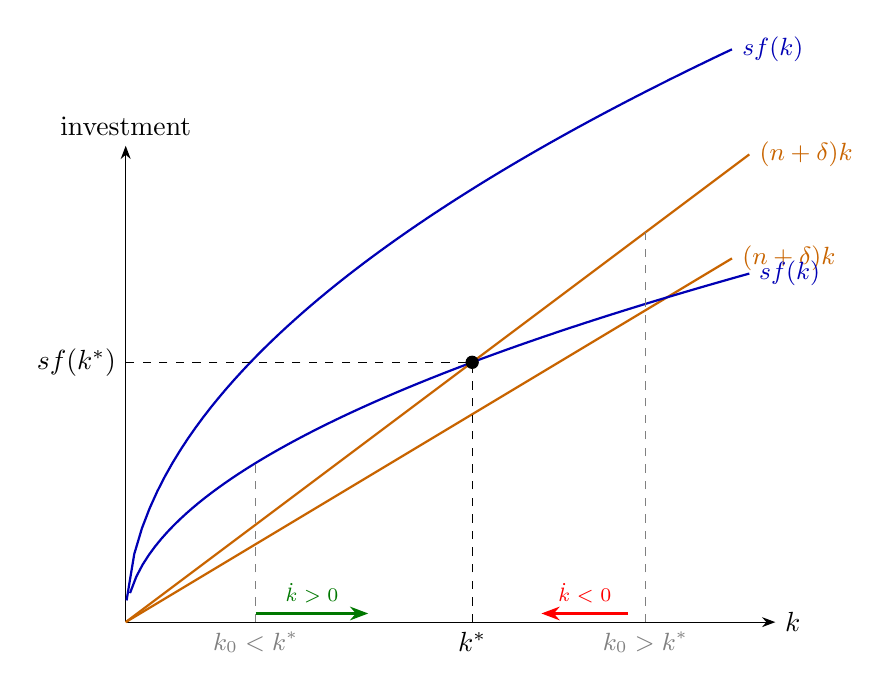
\begin{tikzpicture}[scale=1.1,
    every axis/.style={},
    >=Stealth]

% Axes
\draw[->] (0,0) -- (7.5,0) node[right] {$k$};
\draw[->] (0,0) -- (0,5.5) node[above] {investment};

% Break-even line: (n+delta)*k
\draw[thick, orange3] (0,0) -- (7,4.2)
    node[right, font=\small] {$(n+\delta)k$};

% sf(k) curve: s*k^alpha, approximate with a concave curve
\draw[thick, blue3, domain=0.01:7, samples=80]
    plot (\x, {2.5*\x^0.5})
    node[right, font=\small] {$sf(k)$};

% Steady state: intersection at k* where 2.5*sqrt(k*)=(n+delta)*k*
% 2.5/sqrt(k*) = 0.6 => k* = (2.5/0.6)^2 = 17.36... too big
% Let me set slope = 0.5 for the line
% 2.5*sqrt(k) = 0.5*k => 2.5 = 0.5*sqrt(k) => sqrt(k)=5 => k=25... too big
% Use y=1.8*x^0.45 and line slope 0.55
% intersection: 1.8*k^0.45 = 0.55*k => 1.8 = 0.55*k^0.55 => k^0.55 = 3.27 => k = 3.27^(1/0.55)=7.1
% Let's just pick k*=4 visually

% Redefine: use sf(k) = 1.5*k^0.5, break-even = 0.75*k
% intersection: 1.5*sqrt(k) = 0.75*k => 2 = sqrt(k) => k=4, y=3
\draw[thick, blue3, domain=0.05:7.2, samples=100]
    plot (\x, {1.5*\x^0.5});
% Overwrite with correct curve label (move label up)
\node[blue3, right, font=\small] at (7.2, {1.5*7.2^0.5}) {$sf(k)$};

% Overwrite the orange line with correct slope
\draw[thick, orange3] (0,0) -- (7.2, {0.75*7.2})
    node[right, font=\small] {$(n+\delta)k$};

% k* = 4, y* = 3
\draw[dashed] (4,0) node[below] {$k^*$} -- (4,3) -- (0,3)
    node[left] {$sf(k^*)$};

% Dot at steady state
\filldraw[black] (4,3) circle (2pt);

% Arrows showing convergence
% Left of k*: sf(k) > (n+d)k => k increasing
\draw[->, thick, green3] (1.5,0.1) -- (2.8,0.1)
    node[midway, above, font=\scriptsize, green3] {$\dot{k}>0$};
% Right of k*: sf(k) < (n+d)k => k decreasing
\draw[->, thick, red] (5.8,0.1) -- (4.8,0.1)
    node[midway, above, font=\scriptsize, red] {$\dot{k}<0$};

% k_0 left example
\draw[dashed, gray] (1.5,0) node[below, gray, font=\small] {$k_0 < k^*$}
    -- (1.5, {1.5*1.5^0.5});

% k_0 right example
\draw[dashed, gray] (6,0) node[below, gray, font=\small] {$k_0 > k^*$}
    -- (6, {0.75*6});

\end{tikzpicture}
\end{center}

\subsection*{Reading the Phase Diagram}

\begin{itemize}
    \item \textbf{Above the intersection} ($k < k^*$): $sf(k) > (n+\delta)k$, so $\dot{k} > 0$ (capital accumulates).
    \item \textbf{Below the intersection} ($k > k^*$): $sf(k) < (n+\delta)k$, so $\dot{k} < 0$ (capital decumulates).
    \item The Inada conditions guarantee $sf(k) > (n+\delta)k$ for small $k$ and $sf(k) < (n+\delta)k$ for large $k$.
    \item The steady state $k^*$ is \textbf{globally stable}.
\end{itemize}

%% ============================================================
\section{Speed of Convergence}
%% ============================================================

\subsection*{Log-Linearization Around Steady State}

\begin{derivationbox}
Let $\hat{k}_t = \ln k_t - \ln k^*$ (log deviation from steady state).

\textbf{Step 1.} The law of motion is $\dot{k} = sf(k) - (n+\delta)k$.

\textbf{Step 2.} Define $\phi(k) \equiv \dot{k}$. At $k^*$, $\phi(k^*) = 0$. Taylor-expand:
\[
\dot{k}_t \approx \phi'(k^*)(k_t - k^*)
\]

\textbf{Step 3.} Compute $\phi'(k^*)$:
\[
\phi'(k) = sf'(k) - (n+\delta)
\]
At steady state, $sf(k^*) = (n+\delta)k^*$, so $s = (n+\delta)k^*/f(k^*)$. Thus:
\[
\phi'(k^*) = (n+\delta)\frac{k^* f'(k^*)}{f(k^*)} - (n+\delta) = (n+\delta)\bigl[\varepsilon_{f,k}(k^*) - 1\bigr]
\]
where $\varepsilon_{f,k}(k^*) = k^* f'(k^*)/f(k^*)$ is the elasticity of output w.r.t.\ capital at $k^*$.

\textbf{Step 4.} Under Cobb-Douglas, $f(k) = k^\alpha$ implies $\varepsilon_{f,k} = \alpha$ everywhere:
\[
\phi'(k^*) = (n+\delta)(\alpha - 1) = -(1-\alpha)(n+\delta)
\]
\end{derivationbox}

\begin{resultbox}
\textbf{Speed of convergence:}
\[
\boxed{\beta = (1-\alpha)(n+\delta)}
\]
\textbf{Convergence equation:}
\[
\dot{\hat{k}}_t \approx -\beta \hat{k}_t \implies \hat{k}_t = \hat{k}_0\, e^{-\beta t}
\]
\[
\ln k_t = (1-e^{-\beta t})\ln k^* + e^{-\beta t} \ln k_0
\]
\textbf{Half-life:}
\[
t_{1/2} = \frac{\ln 2}{\beta}
\]
\end{resultbox}

\subsection*{Properties of Beta}

\begin{itemize}
    \item $\beta$ increases with $n$ and $\delta$ (higher dilution $\Rightarrow$ faster convergence).
    \item $\beta$ decreases with $\alpha$ (higher capital share $\Rightarrow$ slower convergence; diminishing returns matter more when $\alpha$ is small).
    \item The saving rate $s$ \textbf{does not} affect $\beta$ under Cobb-Douglas (it affects $k^*$ but not speed of convergence).
    \item With $\alpha \approx 1/3$, $n=0.01$, $\delta=0.05$: $\beta \approx 0.04$ (half-life $\approx 17$ years).
\end{itemize}

\begin{keyformulabox}
\textbf{Growth rate approximation:}
\[
\gamma_{y,t} \equiv \frac{\dot{y}_t}{y_t} \approx \alpha \cdot \frac{\dot{k}_t}{k_t} \approx -\alpha\beta(\ln k_t - \ln k^*)
\approx -\beta(\ln y_t - \ln y^*)
\]
Countries further below their steady state grow faster (\emph{conditional convergence}).
\end{keyformulabox}

%% ============================================================
\section{Empirics: MRW (1992) and Extensions}
%% ============================================================

\subsection*{Mankiw-Romer-Weil (1992) Baseline}

Cross-country regression implied by Solow model:
\[
\ln\!\left(\frac{Y_i}{L_i}\right) = a + \frac{\alpha}{1-\alpha}\ln s_i - \frac{\alpha}{1-\alpha}\ln(n_i + g + \delta) + \varepsilon_i
\]

\begin{itemize}
    \item \textbf{Basic result:} $R^2 \approx 0.6$, but implied $\alpha \approx 0.6$--$0.7$ (too high; true capital share $\approx 1/3$).
    \item \textbf{Problem:} $\alpha \approx 1/3$ requires the coefficient ratio $\approx 0.5$, but data gives $\approx 1.4$.
\end{itemize}

\subsection*{Augmented Solow: Human Capital}

Augment with human capital $H$: $Y = K^\alpha H^\beta (AL)^{1-\alpha-\beta}$.

Let $s_k, s_h$ denote investment rates in physical and human capital. Steady state:
\[
\ln\!\left(\frac{Y}{L}\right) = \ln A_0 + gt + \frac{\alpha}{1-\alpha-\beta}\ln s_k - \frac{\alpha+\beta}{1-\alpha-\beta}\ln(n+g+\delta) + \frac{\beta}{1-\alpha-\beta}\ln s_h
\]

\begin{resultbox}
\textbf{MRW augmented results:} $R^2 \approx 0.8$, implied $\hat{\alpha} \approx \hat{\beta} \approx 1/3$. Consistent with factor shares.
\end{resultbox}

\subsection*{Development Accounting}

Decompose cross-country income differences:
\[
\ln y_i - \ln y_j = \underbrace{\alpha(\ln k_i - \ln k_j)}_{\text{capital}} + \underbrace{(1-\alpha)(\ln h_i - \ln h_j)}_{\text{human capital}} + \underbrace{(\ln A_i - \ln A_j)}_{\text{TFP}}
\]

\textbf{Finding:} TFP differences account for $\sim$50\% of cross-country income variance.

\subsection*{The Lucas Puzzle}

If $Y = K^\alpha L^{1-\alpha}$, the marginal product of capital is:
\[
MPK = \alpha \frac{Y}{K} = \alpha (y/k)
\]
\textbf{Puzzle:} If $y_{\text{US}}/y_{\text{India}} \approx 15$ and $\alpha = 1/3$, then $MPK_{\text{India}}/MPK_{\text{US}} \approx 15^{1-\alpha} \approx 58$. Capital should flow massively to poor countries. It doesn't.

\textbf{Resolutions:} Human capital differences, TFP/institutions, political risk, financial frictions.

%% ============================================================
\section{Extensions: Poverty Traps and Uzawa's Theorem}
%% ============================================================

\subsection*{Poverty Traps}

Standard Solow implies a unique $k^*$. Non-convexities can generate multiple steady states.

\textbf{Two-technology setup:}
\begin{itemize}
    \item Technology A (subsistence): $y = A k^\alpha$ (low productivity)
    \item Technology B (modern): $y = B k^\alpha - \gamma$ where $B > A$, $\gamma > 0$ (fixed cost)
    \item Threshold capital:
    \[
    \ktilde = \left(\frac{\gamma}{B-A}\right)^{1/\alpha}
    \]
\end{itemize}

\begin{resultbox}
\textbf{Poverty trap:}
\begin{itemize}
    \item $k_0 < \ktilde$: economy uses technology A, converges to low $k^*_A$.
    \item $k_0 > \ktilde$: economy uses technology B, converges to high $k^*_B$.
    \item \textbf{"Big Push":} coordinated investment to push $k_0 > \ktilde$.
\end{itemize}
The $sf(k)$ curve is non-concave and crosses the break-even line multiple times.
\end{resultbox}

\subsection*{Uzawa's Theorem}

\textbf{Question:} What restrictions does a BGP impose on the production function?

\begin{resultbox}
\textbf{Uzawa's Theorem:} On a BGP with $\gamma_Y = n+g > 0$ and $\gamma_K > 0$, the production function must be asymptotically \textbf{labor-augmenting (Harrod-neutral)}:
\[
Y = F(K, AL)
\]
Capital-augmenting or Hicks-neutral technical progress is inconsistent with a BGP (unless $\sigma = 1$, i.e., Cobb-Douglas).
\end{resultbox}

\textbf{Proof sketch:} On BGP, $K/Y$ is constant. With constant $r = F_K$, this requires $F_K$ to depend only on $K/Y$ or equivalently $K/(AL)$, which forces labor augmentation.

\textbf{Implication:} The standard form $Y = F(K, A_t L_t)$ is not merely a convention but a requirement for balanced growth.

%% ============================================================
\section{Problem-Solving Templates}
%% ============================================================

\subsection*{Template 1: Find Steady State}

\begin{enumerate}
    \item Write law of motion: $\dot{k} = sf(k) - (n+\delta)k$
    \item Set $\dot{k}=0$: $sf(k^*) = (n+\delta)k^*$
    \item For Cobb-Douglas: $sk^{*\alpha} = (n+\delta)k^*$, solve for $k^*$
    \item Find $y^* = f(k^*)$, $c^* = (1-s)y^*$
\end{enumerate}

\subsection*{Template 2: Comparative Statics}

Use the steady-state condition implicitly:
\[
s f(k^*) = (n+\delta) k^*
\]
Differentiate both sides with respect to the parameter of interest. E.g., for $\partial k^*/\partial s$:
\[
f(k^*) + s f'(k^*)\frac{\partial k^*}{\partial s} = (n+\delta)\frac{\partial k^*}{\partial s}
\implies
\frac{\partial k^*}{\partial s} = \frac{f(k^*)}{(n+\delta) - sf'(k^*)} > 0
\]
(positive because the denominator equals $(n+\delta)(1-\varepsilon_{f,k}) > 0$).

\subsection*{Template 3: Growth Accounting}

\[
\frac{\dot{Y}}{Y} = \alpha \frac{\dot{K}}{K} + (1-\alpha)\frac{\dot{L}}{L} + \frac{\dot{A}}{A}
\]
\[
\text{TFP growth} = \frac{\dot{A}}{A} = \frac{\dot{Y}}{Y} - \alpha \frac{\dot{K}}{K} - (1-\alpha)\frac{\dot{L}}{L}
\]

\subsection*{Template 4: Speed of Convergence Calculation}

Given $\alpha$, $n$, $\delta$:
\begin{enumerate}
    \item Compute $\beta = (1-\alpha)(n+\delta+g)$ (with technology growth $g$)
    \item Half-life: $t_{1/2} = \ln(2)/\beta \approx 0.693/\beta$
    \item Convergence fraction after $T$ years: $1 - e^{-\beta T}$
\end{enumerate}

\subsection*{Template 5: Golden Rule}

\begin{enumerate}
    \item Write $c^* = f(k^*) - (n+\delta)k^*$
    \item Maximize: $f'(k^*) = n+\delta$
    \item Under Cobb-Douglas: $\alpha k^{*\alpha-1} = n+\delta$, and $s_g = \alpha$
    \item Check: if current $s > \alpha$, dynamically inefficient
\end{enumerate}

%% ============================================================
\section{Common Pitfalls}
%% ============================================================

\begin{enumerate}[label=\textbf{P\arabic*.}]

    \item \textbf{Confusing $k = K/L$ vs.\ $\ktilde = K/(AL)$:}
    The break-even rate for $k$ is $(n+\delta)$; for $\ktilde$ it is $(n+g+\delta)$. Never mix them.

    \item \textbf{Exponent in Cobb-Douglas steady state:}
    \[
    k^* = \left(\frac{s}{n+\delta}\right)^{1/(1-\alpha)} \quad \text{NOT} \quad \left(\frac{s}{n+\delta}\right)^{1/\alpha}
    \]

    \item \textbf{Speed of convergence formula:}
    $\beta = (1-\alpha)(n+\delta)$ for $k$, but $\beta = (1-\alpha)(n+g+\delta)$ for $\ktilde$.

    \item \textbf{Saving rate and convergence:}
    $s$ does NOT affect $\beta$ (Cobb-Douglas). A higher $s$ raises $k^*$ but not the speed of convergence.

    \item \textbf{Dynamic inefficiency direction:}
    Overaccumulation ($s > s_g = \alpha$) is dynamically \emph{in}efficient. Underaccumulation ($s < \alpha$) is dynamically \emph{efficient}.

    \item \textbf{Golden Rule vs.\ Modified Golden Rule:}
    The Solow Golden Rule is $f'(k^*) = n+\delta$. The Ramsey Modified Golden Rule is $f'(k^*) = \rho + \delta$ (different condition — do not confuse).

    \item \textbf{Per-worker vs.\ per-capita:}
    If some fraction of population does not work, adjust accordingly. Usually $L$ = workers = population in Solow.

    \item \textbf{BGP requires technology growth:}
    On BGP, $y$ grows at rate $g$, not at zero. Stagnant BGP only if $g=0$.

    \item \textbf{Log-linearization sign:}
    $\dot{\hat{k}} = -\beta \hat{k}$ means $\hat{k}$ decays toward zero, confirming stability. If you get $+\beta$, check signs.

    \item \textbf{Inada conditions and phase diagram:}
    $\lim_{k\to 0} sf'(k) = \infty > n+\delta$ ensures $sf(k)$ is above $(n+\delta)k$ near origin. Always verify this for non-Cobb-Douglas cases.

\end{enumerate}

%% ============================================================
\section{Quick Reference Formulas}
%% ============================================================

\begin{keyformulabox}[title={Quick Reference: Solow Model}]
\textbf{Laws of Motion:}
\begin{align*}
\dot{k} &= sf(k) - (n+\delta)k \tag{per worker} \\
\dot{\ktilde} &= sf(\ktilde) - (n+g+\delta)\ktilde \tag{per eff.\ worker}
\end{align*}

\textbf{Steady States (Cobb-Douglas $f(k)=k^\alpha$):}
\begin{align*}
k^* &= \left(\tfrac{s}{n+\delta}\right)^{1/(1-\alpha)}, \quad
y^* = \left(\tfrac{s}{n+\delta}\right)^{\alpha/(1-\alpha)} \\
\ktilde^* &= \left(\tfrac{s}{n+g+\delta}\right)^{1/(1-\alpha)}
\end{align*}

\textbf{Golden Rule:}
\begin{align*}
f'(k_g^*) &= n+\delta, \quad s_g = \alpha \text{ (Cobb-Douglas)}
\end{align*}

\textbf{Speed of Convergence:}
\begin{align*}
\beta &= (1-\alpha)(n+\delta), \quad t_{1/2} = \frac{\ln 2}{\beta}
\end{align*}

\textbf{MRW Income Equation:}
\begin{align*}
\ln(Y/L) &= \ln A_0 + gt + \frac{\alpha}{1-\alpha}\ln s - \frac{\alpha}{1-\alpha}\ln(n+g+\delta)
\end{align*}

\textbf{MRW Augmented (with human capital $\beta_H$):}
\begin{align*}
\ln(Y/L) &\propto \frac{\alpha}{1-\alpha-\beta_H}\ln s_k + \frac{\beta_H}{1-\alpha-\beta_H}\ln s_h - \frac{\alpha+\beta_H}{1-\alpha-\beta_H}\ln(n+g+\delta)
\end{align*}

\textbf{Growth Accounting:}
\begin{align*}
\dot{A}/A &= \dot{Y}/Y - \alpha\,\dot{K}/K - (1-\alpha)\,\dot{L}/L
\end{align*}

\textbf{Poverty Trap Threshold:}
\begin{align*}
\ktilde &= \left(\frac{\gamma}{B-A}\right)^{1/\alpha}
\end{align*}
\end{keyformulabox}

\begin{resultbox}[title={BGP Growth Rates Summary}]
\begin{center}
\begin{tabular}{lcc}
\toprule
Variable & Per worker & Aggregate \\
\midrule
$K/L$, $Y/L$, $C/L$ & $g$ & $n+g$ \\
$r$ (return to capital) & $0$ & $0$ \\
$w$ (real wage) & $g$ & $n+g$ \\
\bottomrule
\end{tabular}
\end{center}
\end{resultbox}

\end{document}
